% =====================================================================
%  BEV-VAWA-Lite — Full Bilingual (EN / 中文) Technical Report
%  Compile with: tectonic -X compile paper/full_report.tex
% =====================================================================
\documentclass[11pt,a4paper]{article}

\usepackage[margin=2.2cm]{geometry}
\usepackage{fontspec}
\usepackage{xeCJK}
\setCJKmainfont{Songti SC}
\setCJKsansfont{STHeiti}
\setmainfont{Times New Roman}
\setsansfont{Helvetica}

\usepackage{amsmath,amssymb,mathtools}
\usepackage{booktabs}
\usepackage{array}
\usepackage{graphicx}
\graphicspath{{../results/}{./}}
\usepackage{float}
\usepackage{xcolor}
\usepackage{titlesec}
\usepackage{enumitem}
\usepackage{algorithm}
\usepackage{algpseudocode}
\usepackage[hidelinks]{hyperref}
\usepackage{caption}
\captionsetup{font=small,labelfont=bf}

% natbib-style aliases -- we have no .bib, use plain \cite to the bibitems.
\providecommand{\citep}[1]{\cite{#1}}
\providecommand{\citet}[1]{\cite{#1}}

\definecolor{zhcol}{RGB}{40,40,40}
\definecolor{boxcol}{RGB}{245,245,245}
\definecolor{rulecol}{RGB}{120,120,120}

% ---- bilingual helpers -------------------------------------------------
% English paragraph then Chinese paragraph, visually distinguished with a
% small vertical skip. English in normal black, Chinese slightly indented.
\newcommand{\en}[1]{\par\noindent #1\par\vspace{0.15em}}
\newcommand{\zh}[1]{\par\noindent\color{zhcol}\hspace{0.5em}#1\par\color{black}\vspace{0.6em}}

% bilingual section title helper
\newcommand{\bisec}[2]{\section[#1]{#1\quad\normalfont\small\color{zhcol}\textsf{#2}}}
\newcommand{\bisubsec}[2]{\subsection[#1]{#1\quad\normalfont\small\color{zhcol}\textsf{#2}}}
\newcommand{\bisubsubsec}[2]{\subsubsection[#1]{#1\quad\normalfont\small\color{zhcol}\textsf{#2}}}

\titleformat*{\section}{\Large\bfseries}
\titleformat*{\subsection}{\large\bfseries}
\titleformat*{\subsubsection}{\normalsize\bfseries}

% shorthand math ops
\DeclareMathOperator*{\argmax}{arg\,max}
\DeclareMathOperator*{\argmin}{arg\,min}
\newcommand{\R}{\mathbb{R}}
\newcommand{\bz}{\mathbf{z}}

\title{\textbf{BEV-VAWA-Lite}\\[2pt]
       \normalsize A Lightweight BEV-Native Vision-Action / World-Action Framework\\
       for Indoor PointGoal Navigation\\[4pt]
       \normalsize\color{zhcol}\textsf{面向室内 PointGoal 导航的轻量级 BEV-原生 视觉-动作 / 世界-动作 框架}\\[10pt]
       \large Complete Technical Report \quad\color{zhcol}\textsf{完整技术报告}}
\author{Research Log — BEV-VAWA-Lite Project\\
        \small \texttt{bev-vawa-lite} repository}
\date{April 2026}

\begin{document}
\maketitle

% =====================================================================
\begin{abstract}\noindent
\textbf{EN.} BEV-VAWA-Lite is a depth-only PointGoal navigation stack that
fuses a reactive Vision-Action (VA) branch with a short-horizon latent
World-Action (WA) branch over a shared bird's-eye-view (BEV) state, trained
end-to-end on a consumer Apple M4 laptop. This report documents
(1) the problem formulation and the full architecture,
(2) the mathematical objects behind each module
(geometry lift, candidate fan, latent rollout, analytic fusion rule),
(3) the three-stage curriculum and the depth-only reactive safety layer, and
(4) the experimental protocol on the PIB-Nav MuJoCo benchmark —
including a cross-seed paired analysis demonstrating a robust
$\Delta \text{SR} = +0.093 \pm 0.013$ from the safety layer.
We close with the Gibson PointNav v2 upgrade path that is currently in the
code scaffolding stage and will extend the framework from pseudo-BEV pooling
to a geometrically grounded multi-channel BEV, and from risk-scoring to
latent world-dynamics supervision with a reachability (dead-end) head.

\vspace{0.6em}
\noindent\textbf{中文摘要。}\color{zhcol}
\textsf{BEV-VAWA-Lite 是一个仅使用深度图的 PointGoal 导航系统。它在共享的
鸟瞰图（BEV）状态上融合了一个快速反应的视觉-动作（VA）分支与一个短程隐变
量世界-动作（WA）分支，整体可在一台 Apple M4 消费级笔记本上端到端训练。
本报告系统整理了（1）任务建模与整体架构，（2）各模块背后的数学对象
（几何投影、候选扇形、隐变量短程推演、解析融合规则），（3）三阶段训练课程
与纯深度的反应式安全层，以及（4）在 PIB-Nav / MuJoCo 基准上的实验方案
——含四种子配对分析，表明安全层带来稳健的
$\Delta \mathrm{SR} = +0.093 \pm 0.013$ 提升。文末给出 Gibson PointNav v2
升级路径：将伪 BEV 池化换为几何式三通道 BEV，并将 WA 从纯打分器扩展为含
隐动力学监督 $\mathcal{L}_{\mathrm{dyn}}$ 与可达性（dead-end）头的轻量级
隐空间世界-动作评估器。}\color{black}
\end{abstract}

\noindent\rule{\textwidth}{0.4pt}

% =====================================================================
\bisec{1. Introduction}{引言}

\en{Embodied PointGoal navigation \citep{AndersonOnEvaluation2018} is the
task of moving a robot from a start pose to a metric goal position using
on-board sensing. Recent systems scale to billions of parameters and
multi-GPU training
\citep{InternNav,OmniVLA,NaVILA}, targeting maximum generality across
modalities and environments. This report takes the opposite stance: for the
\emph{static, depth-only, indoor} slice of the problem, a deliberately
lightweight architecture trained on a single consumer laptop is sufficient,
and the useful insight from world models — evaluating candidate actions by
their predicted futures — can be retained in a small latent head rather
than a pixel-level generative model.}

\zh{\textsf{具身 PointGoal 导航任务 \citep{AndersonOnEvaluation2018}是指机器人
通过自身传感器从起点导航到目标位置。近年来相关系统不断规模化，参数量达到十
亿级、需要多 GPU 训练 \citep{InternNav,OmniVLA,NaVILA}，追求跨模态、跨场景
的最大通用性。本报告采取相反的立场：对于\textbf{静态、纯深度、室内}这一切
片任务，一个精心设计的轻量架构在单台消费级笔记本上就足够；同时，\emph{世
界模型}的核心想法——以预测的未来来评价候选动作——可以被一个小型\textbf{隐
空间}头部保留下来，而不必使用像素级生成模型。}}

\en{\textbf{Contributions.}
(i) A BEV-aligned \textbf{VA-WA dual-branch} architecture that separates
fast reactive action proposal from short-horizon latent-space consequence
evaluation.
(ii) A latent \textbf{World-Action head} with $\sim$50\,k parameters that
predicts per-candidate collision risk, goal progress, and an
ensemble-variance uncertainty signal, and which naturally extends to
latent-dynamics and reachability supervision
(\S\ref{sec:future}).
(iii) A \textbf{candidate-generation + analytic re-ranking} mechanism
(5-way anchor fan $+$ $Q_k = \alpha s - \gamma \sigma(r) + \beta p - \delta u$)
that remains interpretable and tuneable without gradient-based RL.
(iv) A \textbf{low-compute experimental protocol} (\emph{PIB-Nav}, a
procedural MuJoCo benchmark) that completes end-to-end — data generation,
three-stage training, closed-loop evaluation — on a laptop, with extensive
ablations and a seed-stability analysis.}

\zh{\textsf{\textbf{贡献。}
（i）基于 BEV 的\textbf{ VA-WA 双分支 }架构，显式区分了快速反应式动作提议
和短程隐空间后果评估；
（ii）参数量约 5 万的\textbf{ 隐空间世界-动作头 }，输出每候选的碰撞风险、
目标进度与集成方差式不确定度，并可自然扩展到隐动力学与可达性监督
（见 \S\ref{sec:future}）；
（iii）\textbf{候选生成 + 解析重排}机制（5 路扇形锚点 +
$Q_k = \alpha s - \gamma \sigma(r) + \beta p - \delta u$ 融合规则），在不
依赖梯度式强化学习的前提下仍保持可解释、可调；
（iv）\textbf{低算力实验方案} ——在 MuJoCo 程序化构造的 PIB-Nav
基准上，数据生成、三阶段训练、闭环评测全部可在笔记本上完成，并配有充分
的消融与种子稳定性分析。}}

% =====================================================================
\bisec{2. Problem Formulation}{问题建模}

\en{A PointGoal navigation episode places a differential-drive robot in a
static indoor room. At step $t$ the agent observes
\[
  o_t \;=\; (\, d_t,\; g_t \,),
  \qquad d_t \in \R^{H \times W},
  \qquad g_t = (r_t, \phi_t) \in \R_{\ge 0} \times [-\pi,\pi),
\]
where $d_t$ is a forward-facing depth image ($128\times128$, FOV $90^\circ$,
truncated at $3.0\,$m) and $g_t$ is the goal in robot-centric polar
coordinates. The action is a linear/angular velocity pair
$a_t = (v_t, \omega_t) \in \R^2$, applied at $10\,$Hz.}

\zh{\textsf{一次 PointGoal 导航 episode 将差速驱动机器人放置于一个静态室
内房间。第 $t$ 步智能体观测
\[
  o_t = (d_t, g_t),\quad
  d_t \in \R^{H\times W},\quad
  g_t = (r_t, \phi_t) \in \R_{\ge 0}\times[-\pi,\pi),
\]
其中 $d_t$ 为前向深度图（$128\times128$、FOV $90^\circ$、$3.0\,$m 截断），
$g_t$ 为以机器人本体坐标系极坐标表达的目标，动作为线速/角速对
$(v_t, \omega_t)$，$10\,$Hz 控制。}}

\en{An episode terminates on any of: (i) reaching the goal within
$0.25\,$m (success), (ii) accumulating $10$ collisions (failure), or
(iii) hitting the $300$-step budget (time-out). Evaluation metrics,
following \citet{AndersonOnEvaluation2018}, are
\[
  \mathrm{SR} = \tfrac{1}{N}\sum_{i} \mathbf{1}[\text{success}_i],
  \qquad
  \mathrm{SPL} = \tfrac{1}{N}\sum_{i} \mathbf{1}[\text{success}_i]\cdot
                 \tfrac{\ell^{\star}_i}{\max(\ell^{\star}_i,\ell^{\text{agent}}_i)},
\]
plus the CollisionRate (fraction of episodes with $\ge 1$ contact) and the
PathLenRatio (agent path length / shortest path length, restricted to
successful episodes with finite reference).}

\zh{\textsf{episode 在以下任一条件下终止：（i）到达目标 $0.25\,$m 以内
（成功）、（ii）累计 $10$ 次碰撞（失败）、（iii）超过 $300$ 步预算
（超时）。评测指标参照 \citet{AndersonOnEvaluation2018}：
\[
  \mathrm{SR} = \tfrac{1}{N}\sum_i \mathbf{1}[\text{成功}_i],\quad
  \mathrm{SPL} = \tfrac{1}{N}\sum_i \mathbf{1}[\text{成功}_i]\cdot
                 \tfrac{\ell^{\star}_i}{\max(\ell^{\star}_i,\ell^{\text{agent}}_i)},
\]
此外还给出 CollisionRate（至少发生一次碰撞的 episode 占比）与
PathLenRatio（成功 episode 的路径长度与最短路径长度之比，排除无效参考路
径情形）。}}

% =====================================================================
\bisec{3. Architecture}{整体架构}

\en{Figure~\ref{fig:arch} shows the data flow. The model factorises into
a \emph{shared} BEV encoder that summarises $(d_t, g_t)$ into a latent
$\bz_t \in \R^{128}$, a \emph{fast} VA branch that proposes $K{=}5$
candidate waypoints, and a \emph{slow} WA branch that evaluates each
candidate's short-horizon latent consequences. An analytic fusion rule
picks the winning candidate; pure-pursuit converts it to $(v_t, \omega_t)$.}

\zh{\textsf{图~\ref{fig:arch} 给出整体数据流。模型被分解为三部分：一个
\textbf{共享}的 BEV 编码器，把 $(d_t, g_t)$ 汇聚为隐向量
$\bz_t \in \R^{128}$；一个\textbf{快速}的 VA 分支，提出 $K{=}5$ 个候选
路径点；以及一个\textbf{慢速}的 WA 分支，评估每个候选在短程隐空间中的后
果。随后由解析融合规则选出获胜候选，再用纯追踪控制器换算成
$(v_t, \omega_t)$。}}

\begin{figure}[H]
  \centering
  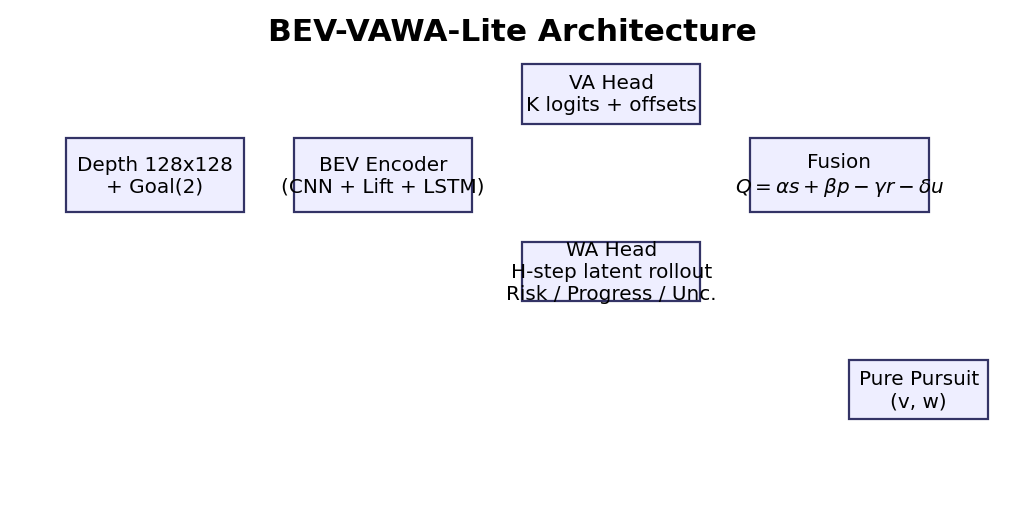
\includegraphics[width=0.85\textwidth]{architecture.png}
  \caption{BEV-VAWA-Lite data flow. \textsf{\small BEV-VAWA-Lite 数据流。}}
  \label{fig:arch}
\end{figure}

\bisubsec{3.1 Shared BEV Encoder}{共享 BEV 编码器}

\en{The encoder consists of a 3-block depth CNN with channel widths
$32{\rightarrow}64{\rightarrow}96$ and $5{\times}5,\,3{\times}3,\,3{\times}3$
kernels at stride 2. The intermediate feature map is lifted to a top-down
feature of resolution $64\times 64$ via adaptive pooling (this is the
``pseudo-BEV'' operator used on the PIB-Nav main line; a geometric
replacement is described in \S\ref{sec:future}). The lifted feature is
concatenated with the embedded goal vector, flattened, and passed through a
\emph{single LSTM cell} to obtain the latent state $\bz_t \in \R^{128}$.
We use an LSTM rather than a GRU because on Apple MPS the GRU CUDA-backed
kernel is missing and the CPU fallback is $\sim 3\times$ slower.}

\zh{\textsf{编码器由 3 段深度 CNN（通道数 $32{\to}64{\to}96$，卷积核分别
$5{\times}5,\,3{\times}3,\,3{\times}3$，步长 2）构成。中间特征通过自适应
池化被提升到 $64\times 64$ 的俯视图（此即 PIB-Nav 主线采用的\textbf{ 伪-BEV
}算子；几何化替代方案见 \S\ref{sec:future}）。俯视图特征与目标向量嵌入拼
接、展平后，通过\textbf{单层 LSTMCell }得到隐状态
$\bz_t \in \R^{128}$。采用 LSTM 而非 GRU 的原因是在 Apple MPS 上 GRU 缺少
CUDA 后端，CPU 回退要慢约 3 倍。}}

\bisubsec{3.2 Vision-Action (VA) Head}{视觉-动作头}

\en{The VA head is a small MLP that reads $\bz_t$ and outputs
(i) $K{=}5$ logits $s_k \in \R$ and
(ii) $K{=}5$ small offset vectors $\Delta_k \in \R^2$, $\|\Delta_k\|_\infty \le 0.3\,$m.
The $K{=}5$ \emph{anchor} waypoints are fixed in robot-centric coordinates
on a $120^\circ$ front-facing fan at radius $R{=}1.5\,$m:
\begin{equation}
  a_k = (R\cos\theta_k,\; R\sin\theta_k),
  \quad \theta_k = -60^\circ + k\cdot 30^\circ,\; k=0,\dots,4.
  \label{eq:anchors}
\end{equation}
The actual per-candidate waypoint passed downstream is $w_k = a_k + \Delta_k$.}

\zh{\textsf{VA 头是一个小型 MLP，从 $\bz_t$ 读出：
（i）$K{=}5$ 个 logits $s_k$；
（ii）$K{=}5$ 个小偏移 $\Delta_k \in \R^2$，$\|\Delta_k\|_\infty \le 0.3\,$m。
$K{=}5$ 个\textbf{锚点}路径点在机器人自身坐标系下固定在半径
$R{=}1.5\,$m 的 $120^\circ$ 前向扇形上（式 \eqref{eq:anchors}）；实际传
给下游的候选点为 $w_k = a_k + \Delta_k$。}}

\bisubsec{3.3 World-Action (WA) Head}{世界-动作头}

\en{For each of the $K$ candidates the WA head performs a short-horizon
rollout. The candidate is embedded
($\mathbb{R}^2 \to \mathbb{R}^{16}$) and consumed, together with the current
latent $\bz_t$, by a \emph{separate} LSTMCell for $H{=}3$ steps. Write
$\hat{\bz}_{t+\tau,k}$ for the hidden state at rollout step $\tau\in\{1,2,3\}$
conditioned on candidate $k$. Three heads read the \emph{final} rollout
hidden state:
\begin{itemize}[leftmargin=1.6em,nosep]
\item \textbf{Risk head} — 3 parallel linear heads form an ensemble of
      binary collision-risk logits. Let
      $\hat r_k = \tfrac{1}{3}\sum_{m=1}^{3} \hat r_k^{(m)}$ be the mean.
\item \textbf{Progress head} — scalar predicting goal-distance reduction
      $\hat p_k \in \R$.
\item \textbf{Uncertainty} — ensemble variance
      $\hat u_k = \mathrm{Var}_m\bigl[\sigma(\hat r_k^{(m)})\bigr]$, no
      separate parameters.
\end{itemize}
The head has roughly $50\,$k parameters — about $4.5\%$ of the total
$1.12\,$M model.}

\zh{\textsf{对每个候选，WA 头进行一次短程推演。候选被嵌入
（$\R^2 \to \R^{16}$）后，与当前隐向量 $\bz_t$ 一起馈入一个\textbf{独立}
的 LSTMCell，展开 $H{=}3$ 步；记 $\hat{\bz}_{t+\tau,k}$ 为条件在候选 $k$
上、第 $\tau$ 步的隐状态。随后三个头从最后一步隐状态读出：
\begin{itemize}[leftmargin=1.6em,nosep]
\item \textbf{风险头}——3 路并行的碰撞二分类 logits 形成集成，均值记作
      $\hat r_k$；
\item \textbf{进度头}——标量 $\hat p_k$，预测目标距离缩减量；
\item \textbf{不确定度}——集成 sigmoid 方差
      $\hat u_k = \mathrm{Var}_m[\sigma(\hat r_k^{(m)})]$，无额外参数。
\end{itemize}
WA 头参数量约 $5$ 万，约占整机 $1.12\,$M 参数的 $4.5\%$。}}

\bisubsec{3.4 Analytic Fusion Rule}{解析融合规则}

\en{Let $\tilde{s}_k = \mathrm{softmax}(s)_k$. Each candidate receives a
score
\begin{equation}
  Q_k \;=\; \alpha\,\tilde{s}_k \;+\; \beta\,\hat{p}_k
        \;-\; \gamma\,\sigma(\hat{r}_k) \;-\; \delta\,\hat{u}_k,
  \label{eq:fusion}
\end{equation}
with fixed weights $(\alpha,\beta,\gamma,\delta)=(1.0,\,1.5,\,2.0,\,0.5)$.
The argmax candidate $k^{\star} = \argmax_k Q_k$ is passed as a goal to a
pure-pursuit controller that outputs $(v_t,\omega_t)$. The weights were
chosen by a short manual grid on the Stage-A checkpoint's validation set;
automating this choice is left to future work.}

\zh{\textsf{记 $\tilde{s}_k = \mathrm{softmax}(s)_k$，则每个候选得分为
\[
  Q_k = \alpha\tilde{s}_k + \beta\hat{p}_k - \gamma\sigma(\hat r_k) - \delta\hat u_k,
\]
固定权重 $(\alpha,\beta,\gamma,\delta) = (1.0,1.5,2.0,0.5)$。argmax
$k^{\star}$ 对应的候选被送入纯追踪控制器产出 $(v_t,\omega_t)$。权重值由
在 Stage-A 验证集上的一次小范围手工格点搜索确定，自动化选择留作未来工
作。}}

% =====================================================================
\bisec{4. Mathematical Details}{数学原理}

\bisubsec{4.1 Geometry Lift (Gibson-v2 track)}{几何投影（Gibson-v2 路线）}

\en{On the Gibson-v2 path the ``adaptive-pool'' pseudo-BEV is replaced by a
differentiable pinhole back-projection. Given depth $d_t(u,v)$ with
calibrated intrinsics $f_x, f_y, c_x, c_y$, each valid pixel $(u,v)$
projects to a 3-D camera-frame point
\[
   X_c = \tfrac{(u - c_x)\,d_t(u,v)}{f_x},\quad
   Y_c = \tfrac{(v - c_y)\,d_t(u,v)}{f_y},\quad
   Z_c = d_t(u,v).
\]
Dropping $Y_c$ (the height) projects the point onto the floor plane,
giving a BEV sample $(x_{\mathrm{bev}}, y_{\mathrm{bev}}) = (Z_c, X_c)$.
Samples outside the grid window $[0,3.0]\times[-1.5,1.5]\,$m or with
$d_t \le d_{\min}$ are masked out. The grid is
$64\times 64$, so the cell size is $\sim 4.7\,$cm $\times$ $4.7\,$cm.}

\zh{\textsf{在 Gibson-v2 路线上，自适应池化的伪-BEV 被替换为可微的针孔反
投影。给定深度 $d_t(u,v)$ 与已校准内参 $f_x, f_y, c_x, c_y$，每个有效像素
$(u,v)$ 投影到相机坐标系下的三维点 $(X_c, Y_c, Z_c)$：
\[
   X_c = \tfrac{(u-c_x)d_t(u,v)}{f_x},\ Y_c = \tfrac{(v-c_y)d_t(u,v)}{f_y},\
   Z_c = d_t(u,v).
\]
舍去高度 $Y_c$ 即投影到地面，得到 BEV 样本
$(x_{\mathrm{bev}}, y_{\mathrm{bev}}) = (Z_c, X_c)$。超出格点窗口
$[0,3.0]\times[-1.5,1.5]\,$m 或 $d_t \le d_{\min}$ 的样本被屏蔽。网格为
$64\times 64$，即每格约 $4.7\,$cm $\times$ $4.7\,$cm。}}

\en{Three output channels are produced:
\textbf{(1)~occ} — $\mathrm{occ}[i,j] = \min\{1, \mathrm{count}[i,j]\}$
via a differentiable \texttt{scatter\_add};
\textbf{(2)~free} — for each depth column we mark cells between the camera
origin and the first-hit cell along its BEV-plane projection with a
discrete Bresenham traversal;
\textbf{(3)~goal~prior} — a truncated Gaussian sector heatmap centred at the
goal bearing $\phi_t$ with $\sigma_{\phi}=0.35\,$rad.
At training time an optional ``channels-enabled'' mask
(\texttt{[1,1,1]} by default) allows single-channel ablations.}

\zh{\textsf{几何提升产出三个通道：
\textbf{（1）occ}——以可微 \texttt{scatter\_add} 得
$\mathrm{occ}[i,j] = \min\{1, \mathrm{count}[i,j]\}$；
\textbf{（2）free}——对每个深度列，在其 BEV 平面投影上用离散
Bresenham 追迹，将相机原点到首次击中格之间的空闲格打上 $1$；
\textbf{（3）goal-prior}——以目标方位 $\phi_t$ 为中心、
$\sigma_{\phi}=0.35\,$rad 的截断高斯扇形热图。
训练时一个可选的 \texttt{channels-enabled} 掩码（默认 \texttt{[1,1,1]}）
可用于通道消融。}}

\bisubsec{4.2 Best-K Supervision and the Huber Offset Loss}{最佳-K 监督与 Huber 偏移损失}

\en{The expert trajectory provides a target waypoint $w^{\star}_t$.
The target anchor index is
\begin{equation}
  k^{\star} \;=\; \argmin_{k=0,\dots,K-1} \|a_k - w^{\star}_t\|_2,
\end{equation}
and VA is trained with cross-entropy on $s$ plus a Huber regression on the
selected candidate's offset:
\begin{equation}
  \mathcal{L}_{\mathrm{VA}} \;=\;
  \underbrace{-\log \tilde{s}_{k^\star}}_{\mathcal{L}_{\mathrm{CE}}}
  \;+\; \lambda_{\mathrm{off}} \cdot
  \underbrace{H_\tau\bigl(w_{k^\star} - w^{\star}_t\bigr)}_{\mathcal{L}_{\mathrm{Huber}}},
  \qquad \lambda_{\mathrm{off}} = 0.5,
\end{equation}
with $H_\tau$ the element-wise Huber loss with knee
$\tau = 0.1\,$m. The rationale for Huber over MSE is outlier robustness
against expert samples near obstacles where the waypoint resampling can
jitter.}

\zh{\textsf{专家轨迹提供目标路径点 $w^{\star}_t$，目标锚点索引为
$k^{\star} = \argmin_k \|a_k - w^{\star}_t\|_2$；VA 的损失为 logits 的交
叉熵加选中候选偏移的 Huber 回归：
\[
 \mathcal{L}_{\mathrm{VA}} = -\log \tilde s_{k^{\star}}
 + \lambda_{\mathrm{off}} H_\tau(w_{k^{\star}} - w^{\star}_t),
 \quad \lambda_{\mathrm{off}}=0.5,\;\tau=0.1\,\mathrm{m}.
\]
选择 Huber 而非 MSE 的理由是：对于专家在障碍边沿的重采样抖动具有更好的鲁
棒性。}}

\bisubsec{4.3 WA Losses}{WA 损失}

\en{For each candidate $k$ we compute labels using the inflated occupancy
grid: $r_k \in \{0,1\}$ (collision between robot pose and $a_k$) and
$p_k \in [-1,1]$ (normalised geodesic-distance reduction to the goal).
The WA loss is
\begin{equation}
  \mathcal{L}_{\mathrm{WA}} \;=\;
  \underbrace{\tfrac{1}{K\cdot M}\sum_{k,m}\mathrm{BCE}\!\bigl(\hat r_k^{(m)}, r_k\bigr)}_{\mathcal{L}_{\mathrm{risk}}}
  \;+\;
  \underbrace{\tfrac{1}{K}\sum_{k} \bigl(\hat p_k - p_k\bigr)^2}_{\mathcal{L}_{\mathrm{prog}}},
\end{equation}
where $M=3$ is the ensemble size. No explicit loss trains $\hat u_k$; it is
defined as the ensemble variance of the sigmoids of $\hat r_k^{(m)}$.}

\zh{\textsf{对每个候选 $k$，利用膨胀占据栅格生成标签：$r_k\in\{0,1\}$（从
当前机器人位姿到 $a_k$ 是否碰撞）与 $p_k\in[-1,1]$（归一化地测距离削减
量）。WA 损失为
\[
 \mathcal{L}_{\mathrm{WA}}
 = \tfrac{1}{KM}\sum_{k,m}\mathrm{BCE}(\hat r_k^{(m)}, r_k)
 + \tfrac{1}{K}\sum_k(\hat p_k - p_k)^2,
\]
其中 $M=3$ 为集成规模；不确定度 $\hat u_k$ 不参与训练，它被定义为集成
sigmoid 的方差。}}

\bisubsec{4.4 Gibson-v2 Extensions: $\mathcal{L}_{\mathrm{dyn}}$ and the Dead-end Head}{Gibson-v2 扩展：$\mathcal{L}_{\mathrm{dyn}}$ 与 dead-end 头}

\en{On the Gibson-v2 path two additional losses are added to supervise the
\emph{intermediate} rollout latents of the WA branch and to introduce
reachability awareness. Let $z^{\mathrm{gt}}_{t+\tau}$ denote the encoder
latent computed (no-grad) from future depth frames $d_{t+\tau}$ obtained
by teleporting the simulator along the resampled expert path. The
latent-dynamics loss is
\begin{equation}
  \mathcal{L}_{\mathrm{dyn}} \;=\;
  \frac{1}{H}\sum_{\tau=1}^{H}
  \bigl\| \hat{\bz}_{t+\tau,k^{\star}} - z^{\mathrm{gt}}_{t+\tau} \bigr\|_2^2,
\end{equation}
applied only to the expert-selected anchor to avoid degenerate
cross-candidate collapse. A dead-end head
$\mathrm{DE}(\hat{\bz}_{t+H,k}) \to d_k \in \R$ is trained on a binary
label $\ell^{\mathrm{DE}}_k \in \{0,1\}$ produced by
\texttt{pathfinder.find\_path} after a candidate teleport — label $=1$
iff there is no navigable path from the candidate endpoint to the goal.
Its loss is
$\mathcal{L}_{\mathrm{DE}} = \tfrac{1}{K}\sum_k \mathrm{BCE}(d_k, \ell^{\mathrm{DE}}_k)$.
Fusion is extended to
\(
  Q_k^{\mathrm{v2}} = Q_k - \eta\,\sigma(d_k)
\)
with $\eta = 1.0$.}

\zh{\textsf{Gibson-v2 路线额外引入两个损失，用于监督 WA 分支的\textbf{中
间 }推演隐状态，并引入可达性意识。记 $z^{\mathrm{gt}}_{t+\tau}$ 为在专家
重采样路径上前进 $\tau$ 步、对该处深度帧做无梯度编码得到的“未来真值隐
向量”。隐动力学损失为
\[
 \mathcal{L}_{\mathrm{dyn}}
 = \tfrac{1}{H}\sum_\tau \|\hat{\bz}_{t+\tau,k^{\star}} - z^{\mathrm{gt}}_{t+\tau}\|_2^2,
\]
仅在\textbf{专家锚点}上施加，避免跨候选坍缩。
dead-end 头 $\mathrm{DE}(\hat{\bz}_{t+H,k}) \to d_k$ 训练于 Habitat
\texttt{pathfinder.find\_path} 生成的二分标签
$\ell^{\mathrm{DE}}_k$（候选点到目标是否仍可达）：
$\mathcal{L}_{\mathrm{DE}} = \tfrac{1}{K}\sum_k \mathrm{BCE}(d_k, \ell^{\mathrm{DE}}_k)$。融合规则扩展为
$Q_k^{\mathrm{v2}} = Q_k - \eta\sigma(d_k)$，$\eta=1.0$。}}

\bisubsec{4.5 Pure-Pursuit Controller}{纯追踪控制器}

\en{Given a selected candidate $w = (x_w, y_w)$ expressed in robot-centric
coordinates, the pure-pursuit rule \citep{Coulter1992} outputs
\begin{equation}
  \omega \;=\; \frac{2\,v\,y_w}{x_w^2 + y_w^2},
  \qquad
  v \;=\; \min\!\Bigl(v_{\max},\; k_v \sqrt{x_w^2 + y_w^2}\Bigr),
\end{equation}
with $k_v = 0.8$ and $v_{\max} = 0.4\,$m/s. The form is algebraic, has
no learnable parameters, and introduces a controller-level bottleneck that
shows up in the A$^\star$ upper bound (\S\ref{sec:results}).}

\zh{\textsf{给定机器人坐标系下的路径点 $w=(x_w,y_w)$，纯追踪控制
\citep{Coulter1992} 给出
\[
 \omega = \tfrac{2 v y_w}{x_w^2 + y_w^2},\quad
 v = \min(v_{\max}, k_v\sqrt{x_w^2 + y_w^2}),
\]
$k_v=0.8$，$v_{\max}=0.4\,$m/s。该形式为代数式、无可学习参数，但会构成
\textbf{控制器层面}的瓶颈，这在 A$^\star$ 上限中明显可见
（见 \S\ref{sec:results}）。}}

% =====================================================================
\bisec{5. Training Pipeline}{训练流程}

\bisubsec{5.1 Data Generation (PIB-Nav)}{数据生成（PIB-Nav）}

\en{\textsf{PIB-Nav} is a procedural MuJoCo-based benchmark built for this
project. Rooms are axis-aligned rectangles of uniformly sampled side in
$[5,7]\,$m, populated with $U(3,6)$ obstacles of uniformly sampled
side $[0.4,1.2]\,$m. The robot is a differential-drive base of radius
$0.20\,$m with a forward-facing $128\times 128$ depth camera.}

\zh{\textsf{\textbf{PIB-Nav} 是本项目为本工作构建的一个 MuJoCo 程序化导
航基准。房间为轴对齐矩形，边长在 $[5,7]\,$m 均匀采样，内含 $U(3,6)$ 个
障碍物，障碍边长在 $[0.4,1.2]\,$m 均匀采样。机器人半径 $0.20\,$m，差速
驱动，配备 $128\times 128$ 前向深度相机。}}

\en{For each of $1000$ procedural rooms we sample $64$ training poses as
follows: (i) A$^\star$-plan a collision-free path on the inflated
occupancy grid; (ii) Chaikin-smooth twice; (iii) resample at arclength
$0.1\,$m; (iv) at each chosen arclength, teleport the robot to the pose
with small Gaussian noise and render depth. Per-sample labels are:
expert waypoint $w^{\star}_t = $ path point $1.5\,$m ahead, best-$k^{\star}$
index, and per-candidate $(r_k, p_k)$ from the occupancy grid. Total
dataset size: $64{,}000$ samples, generated in $\sim 5.5\,$h on the M4
laptop. Shards are written as \texttt{.npz} files, one per room.}

\zh{\textsf{对每个 $1000$ 个房间，按如下步骤采集 $64$ 个样本：
（i）在膨胀占据栅格上 A$^\star$ 规划出一条无碰撞路径；
（ii）做两次 Chaikin 平滑；
（iii）按弧长 $0.1\,$m 重采样；
（iv）在每个采样点，把机器人瞬移到该位姿（带小高斯噪声）并渲染深度。
每样本的监督标签包括：前瞻 $1.5\,$m 的专家路径点 $w^{\star}_t$、
最佳 $k^{\star}$ 索引，以及候选级 $(r_k, p_k)$ 标签（由占据栅格生成）。
数据集总规模 $64{,}000$ 样本，在 M4 上耗时约 $5.5$ 小时生成；每个房间为
一个 \texttt{.npz} 分片。}}

\bisubsec{5.2 Three-Stage Curriculum}{三阶段训练课程}

\en{\textbf{Stage A — VA supervision.} The encoder plus VA head are
trained with $\mathcal{L}_{\mathrm{VA}}$ on all samples for $20$ epochs.
\textbf{Stage B — WA supervision.} The Stage-A encoder is \emph{frozen}
and the WA head is trained with $\mathcal{L}_{\mathrm{WA}}$ for $20$
epochs; on the Gibson-v2 path $\mathcal{L}_{\mathrm{dyn}}$ and
$\mathcal{L}_{\mathrm{DE}}$ are added with weights $0.5$.
\textbf{Stage C — joint fine-tune.} The last encoder block and both heads
are unfrozen and trained together for $8$ epochs with the joint loss; on
Gibson-v2 the $\mathcal{L}_{\mathrm{dyn}}$ / $\mathcal{L}_{\mathrm{DE}}$
weights are reduced to $0.2$ to stabilise joint optimisation.
Optimiser: AdamW, $\mathrm{lr}=3\mathrm{e}{-4}$,
$\mathrm{wd}=1\mathrm{e}{-5}$, grad-clip $1.0$, batch size $64$.
Total wall-clock training on the M4: $\sim 3\,$h.}

\zh{\textsf{\textbf{Stage A——VA 监督：}用 $\mathcal{L}_{\mathrm{VA}}$
联合训练编码器与 VA 头 $20$ epoch。
\textbf{Stage B——WA 监督：}冻结 Stage-A 编码器，只训练 WA 头 $20$ epoch；
Gibson-v2 路线再加入 $\mathcal{L}_{\mathrm{dyn}}$ 与
$\mathcal{L}_{\mathrm{DE}}$，权重 $0.5$。
\textbf{Stage C——联合微调：}解冻编码器最后一段和两头部，联合损失训练
$8$ epoch；Gibson-v2 路线把 $\mathcal{L}_{\mathrm{dyn}}$、
$\mathcal{L}_{\mathrm{DE}}$ 的权重降到 $0.2$ 以稳定联合优化。
优化器 AdamW，$\mathrm{lr}=3\mathrm{e}{-4}$，
$\mathrm{wd}=1\mathrm{e}{-5}$，梯度裁剪 $1.0$，batch 64；M4 整套训练约
$3$ 小时。}}

\begin{algorithm}[H]
\caption{Three-Stage Training \textsf{\small 三阶段训练}}
\begin{algorithmic}[1]
\State initialise encoder $E$, VA head $V$, WA head $W$
\For{epoch $= 1,\dots,20$} \Comment{Stage A}
  \State update $E, V$ with $\mathcal{L}_{\mathrm{VA}}$
\EndFor
\State freeze $E$
\For{epoch $= 1,\dots,20$} \Comment{Stage B}
  \State update $W$ with $\mathcal{L}_{\mathrm{WA}}$\quad ($+\,\mathcal{L}_{\mathrm{dyn}}, \mathcal{L}_{\mathrm{DE}}$ on Gibson-v2)
\EndFor
\State unfreeze last block of $E$
\For{epoch $= 1,\dots,8$} \Comment{Stage C}
  \State update $\{E_{\text{last}}, V, W\}$ with joint loss
\EndFor
\end{algorithmic}
\end{algorithm}

% =====================================================================
\bisec{6. Reactive Safety Layer (v3)}{反应式安全层 (v3)}

\en{\textbf{Motivation.} Inspection of the 55 failures of the Stage-C
checkpoint at seed $12345$ showed $\sim 95\%$ were collision-budget
exhaustion, not time-outs or goal divergence. The residual failures are
amenable to a purely \emph{reactive} override that never rewrites the
policy's training signal.}

\zh{\textsf{\textbf{动机。}在种子 $12345$ 上，Stage-C 检查点的 $55$ 次失败
中约 $95\%$ 是碰撞预算耗尽，而非超时或目标偏离。剩余失败对一个纯反应式
\textbf{外挂模块}是高度可纠正的，后者不需要改动训练信号。}}

\en{\textbf{Design.} At each step the safety layer observes $d_t$ and the
policy's proposed $(v,\omega)$, and outputs a modified $(v', \omega')$.
Depth pixels outside the valid range are discarded. Statistics use the
$5^{\mathrm{th}}$ percentile to be robust to MuJoCo depth misses.}

\zh{\textsf{\textbf{设计。}每步安全层观测 $d_t$ 与策略给出的 $(v,\omega)$，
输出修正后的 $(v',\omega')$。越界深度像素先被丢弃，关键统计量取剩余像素
的 $5$ 百分位，以抵抗 MuJoCo 偶发的深度缺失。}}

\en{\emph{Forward APF.} Define the forward band as the middle
$60\%$ ($\pm 27^\circ$ at FOV $90^\circ$) of columns and the middle
$40\%$ of rows. Let $d_{\min}$ be the $5$th-percentile clearance in this
band. When $d_{\min} < d_{\mathrm{warn}} = 0.60\,$m we emit a forward
correction proportional to left-right asymmetry $a \in [-1,1]$ and an
urgency ramp $\kappa = \mathrm{clip}((d_{\mathrm{warn}}-d_{\min})/(d_{\mathrm{warn}}-d_{\mathrm{near}}),0,1)$,
with $d_{\mathrm{near}} = 0.35\,$m:
\begin{equation}
  \omega_{\mathrm{fwd}} \;=\; a\cdot \omega_{\max}\cdot(0.5 + 0.5\,\kappa).
\end{equation}
A fallback sign (policy's own $\omega$, then a fixed left bias) prevents
spin-in-place lock when $|a|$ is below a tiebreaker threshold.}

\zh{\textsf{\emph{前向 APF。}定义前向带为列方向 $60\%$（FOV 下约
$\pm 27^\circ$）、行方向 $40\%$ 的中心区域。记 $d_{\min}$ 为该区域剩余像素
的 $5$ 百分位净距。当 $d_{\min} < d_{\mathrm{warn}} = 0.60\,$m 时，根据左
右不对称度 $a \in [-1,1]$ 与紧迫度
$\kappa = \mathrm{clip}((d_{\mathrm{warn}}-d_{\min})/(d_{\mathrm{warn}}-d_{\mathrm{near}}),0,1)$
（$d_{\mathrm{near}}=0.35\,$m）输出前向修正
$\omega_{\mathrm{fwd}} = a\omega_{\max}(0.5+0.5\kappa)$；当 $|a|$ 小于阈值
时回退到策略自身的 $\omega$ 方向，再退化为固定左偏，避免原地自旋。}}

\en{\emph{Lateral scrape guard.} The forward arc alone is blind to
episodes where the front is clear but the shoulder grazes an obstacle
during a turn. We add two lateral sectors covering the outer $20\%$ of
columns on each side, with closeness scores
$c_\ell, c_r \in [0,1]$ derived from the same statistic and a side warning
distance $d_{\mathrm{side}}=0.40\,$m. The side correction is always
evaluated and summed with the forward term; a mild speed taper is applied:
\begin{equation}
  \omega_{\mathrm{side}} = (c_r - c_\ell)\,g\,\omega_{\max},\qquad
  v_{\mathrm{mult}} = 1 - (1-\tau_v)\max(c_\ell, c_r),
\end{equation}
\begin{equation}
  \omega' = \mathrm{clip}(\omega + \omega_{\mathrm{fwd}} + \omega_{\mathrm{side}},\,
                          -\omega_{\max},\,+\omega_{\max}),
  \qquad
  v' = v_{\mathrm{new}}\cdot v_{\mathrm{mult}},
\end{equation}
with $(g, \tau_v) = (0.6, 0.85)$. Importantly, linear velocity is
\emph{never zeroed} in the innermost band — the controller still advances
at $v = 0.3\,v_{\max}$ while rotating, which empirically eliminates the
``spin-in-place'' lock mode that plagued earlier safety variants.}

\zh{\textsf{\emph{侧向擦碰保护。}仅靠前向弧无法覆盖“前方开阔但肩部在转
弯时擦障”的 episode。为此我们引入两个侧向扇区，各覆盖左右外侧 $20\%$
列，依据相同统计量定义贴近度 $c_\ell, c_r \in [0,1]$，侧向告警距离
$d_{\mathrm{side}}=0.40\,$m。侧向修正\textbf{恒定求值}并与前向项相加，且
附带速度轻度缩减：
\[
 \omega_{\mathrm{side}} = (c_r - c_\ell)g\omega_{\max},\
 v_{\mathrm{mult}} = 1 - (1-\tau_v)\max(c_\ell, c_r),
\]
$(g,\tau_v)=(0.6,0.85)$。关键设计：在\textbf{最内 danger 带}中线速仍保持
$v = 0.3 v_{\max}$ 边转边走，经验上彻底消除了早期安全版本中的“原地自旋死
锁”。}}

% =====================================================================
\bisec{7. Experimental Setup}{实验设置}

\en{\textbf{Benchmark.} PIB-Nav test suite: $100$ procedural rooms held
out from training, seeded. Success threshold $0.25\,$m, collision budget
$10$, step budget $300$.}

\zh{\textsf{\textbf{基准。}PIB-Nav 测试集：$100$ 个测试房间（从训练池中独
立采样），按种子确定。成功阈值 $0.25\,$m，碰撞预算 $10$，步预算 $300$。}}

\en{\textbf{Methods under comparison.}
\emph{A$^\star$ Upper Bound} (oracle planner replanning on inflated
occupancy every step, tracked by the same pure-pursuit controller),
\emph{A$^\star$ + Safety} (same, with reactive safety layer),
\emph{BEV-VAWA (full)} (the learned model),
\emph{BEV-VAWA + Safety}, and three imitation-style baselines sharing
most of the encoder / training pipeline with our method:
\emph{FPV-BC} (front-pixel CNN $\to$ 5-way discrete action + offset),
\emph{BEV-BC} (same head but fed our BEV latent), and
\emph{BEV-VA} (BEV latent + the VA head, i.e.\ our full model with the
WA branch surgically removed). All three baselines are trained with
the same $20$-epoch Stage-A recipe as the VA head in our model and
evaluated at the same four seeds (see Table~\ref{tab:main}).}

\zh{\textsf{\textbf{对比方法。}
\emph{A$^\star$ 上限}（每步在膨胀占据栅格上重规划并用同一纯追踪控制器跟
踪）、\emph{A$^\star$ + Safety}、\emph{BEV-VAWA（完整模型）}、
\emph{BEV-VAWA + Safety}，以及三个共享大部分编码器 / 训练管线的模仿式基
线：\emph{FPV-BC}（前视像素 CNN $\to$ 5 向离散动作 + 偏移）、
\emph{BEV-BC}（同一头部但输入为我们的 BEV 潜表示）、\emph{BEV-VA}（BEV
潜表示 $+$ VA 头部；即把 WA 分支移除后的完整模型）。三者均与我们模型的
VA 头部共用 $20$ epoch 的 Stage-A 训练配方，并在同样的 $4$ 种子上评测，
见表~\ref{tab:main}。}}

\en{\textbf{Seeds.} For the two learned-policy rows we use four seeds
$\{12345, 42, 7, 31337\}$, $100$ episodes each, and report mean $\pm$
sample standard deviation. A$^\star$ is deterministic: a single evaluation
per configuration. Ablations are run at the single seed $12345$ and
interpreted as \emph{paired deltas} to the full-model row at the same
seed — per-seed offset cancels by construction.}

\zh{\textsf{\textbf{种子。}两行学习策略使用 $4$ 种子
$\{12345, 42, 7, 31337\}$，每种子 $100$ episode，报告 mean $\pm$ 样本标
准差。A$^\star$ 为确定性，每配置一次评测。消融仅在 $12345$ 种子上跑，用
\textbf{同种子配对差}解读——种子偏移自然抵消。}}

% =====================================================================
\bisec{8. Results}{结果}\label{sec:results}

\bisubsec{8.1 Main Table}{主表}

\begin{table}[H]
\centering\small
\caption{Primary closed-loop results on PIB-Nav. Learned-policy rows marked
``mean $4$ seeds'' aggregate $\{12345,42,7,31337\}$; A$^\star$ rows are
deterministic. \textsf{\small 在 PIB-Nav 上的主闭环结果。标有
``mean $4$ seeds'' 的行为 $\{12345,42,7,31337\}$ 四种子均值；A$^\star$
行为确定性评测。}}
\label{tab:main}
\begin{tabular}{lccccc}
\toprule
Method & SR $\uparrow$ & SPL $\uparrow$ & Coll $\downarrow$ & PLR & Lat.\,(ms) \\
\midrule
A$^\star$ Upper Bound          & 0.48 & 0.47 & 0.54 & 0.89 & 2.76 \\
A$^\star$ + Safety             & 0.50 & 0.49 & 0.50 & 0.90 & 2.63 \\
\midrule
\multicolumn{6}{l}{\emph{Imitation / reactive baselines — mean 4 seeds}} \\
FPV-BC (mean 4 seeds)          & $0.35\pm 0.03$ & $0.34\pm 0.03$ & $0.69\pm 0.03$ & 0.94 & 1.56 \\
BEV-BC (mean 4 seeds)          & $0.33\pm 0.04$ & $0.32\pm 0.04$ & $0.69\pm 0.05$ & 0.92 & 4.42 \\
BEV-VA (mean 4 seeds)          & $0.33\pm 0.03$ & $0.32\pm 0.03$ & $0.69\pm 0.04$ & 0.92 & 4.13 \\
\midrule
\multicolumn{6}{l}{\emph{Ablations — single seed 12345, n=100}} \\
BEV-VAWA (no\_wa)              & 0.39 & 0.38 & 0.63 & 0.92 & 6.00 \\
BEV-VAWA (no\_unc)             & 0.45 & 0.44 & 0.58 & 0.92 & 5.57 \\
BEV-VAWA (h1)                  & 0.44 & 0.43 & 0.58 & 0.91 & 5.03 \\
BEV-VAWA (full)                & 0.45 & 0.44 & 0.58 & 0.92 & 5.54 \\
BEV-VAWA (full + Safety)       & 0.53 & 0.52 & 0.50 & 0.91 & 6.05 \\
\midrule
\multicolumn{6}{l}{\emph{Cross-seed — mean 4 seeds}} \\
BEV-VAWA (full, mean 4 seeds)            & $0.40\pm 0.05$ & $0.39\pm 0.05$ & $0.65\pm 0.05$ & 0.92 & 5.76 \\
\textbf{BEV-VAWA (full+Safety, mean 4 seeds)} & $\mathbf{0.49\pm 0.05}$ & $\mathbf{0.49\pm 0.05}$ & $\mathbf{0.57\pm 0.06}$ & 0.92 & 6.11 \\
\bottomrule
\end{tabular}
\end{table}

\begin{figure}[H]
\centering
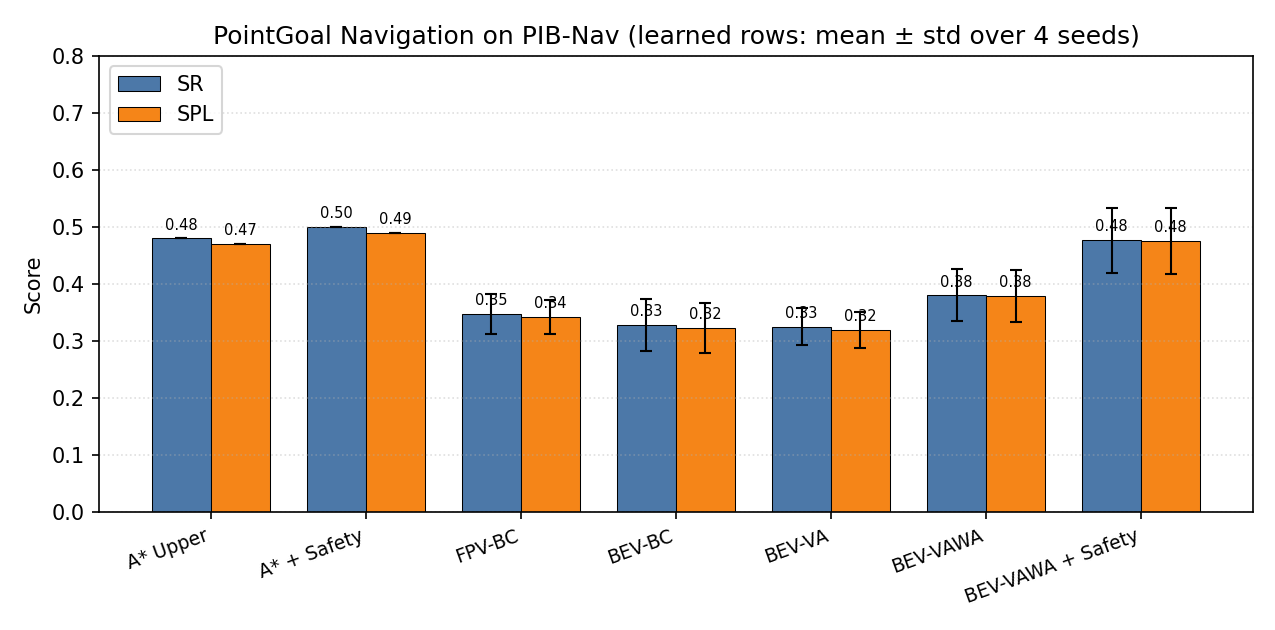
\includegraphics[width=0.80\textwidth]{fig_main_sr_spl.png}
\caption{Main SR/SPL comparison. Learned-policy error bars are
cross-seed $\sigma$. \textsf{\small 主 SR/SPL 对比，学习策略的误差棒为四种子 $\sigma$。}}
\label{fig:main}
\end{figure}

\en{\textbf{Baselines vs.\ our method.} All three imitation baselines cluster
tightly at $\mathrm{SR} \approx 0.33$--$0.35$, essentially indistinguishable
from each other at $n{=}100$. Moving the encoder from raw FPV pixels to the
shared BEV latent (\emph{FPV-BC} $\to$ \emph{BEV-BC}) is neutral; adding the
VA multi-waypoint head (\emph{BEV-BC} $\to$ \emph{BEV-VA}) is also neutral.
It is only when the WA branch contributes a risk / progress / uncertainty
score into the analytic fusion $Q_k$ that SR jumps to
$0.40\pm0.05$, and adding the safety layer lifts it further to
$0.49\pm0.05$. This is consistent with the central claim of the paper:
the WA branch is the component that does load-bearing work, and the
improvement is not attributable to either the BEV lift or the VA head
alone. Latency-wise, all BEV-based variants sit around $4$--$6$\,ms —
well below our real-time budget.}

\zh{\textsf{\textbf{基线对比。}三条模仿基线的 SR 聚集在
$0.33$--$0.35$，在 $n{=}100$ 下彼此基本不可区分。把编码器从原始 FPV
像素换成共享 BEV 潜表示（\emph{FPV-BC} $\to$ \emph{BEV-BC}）是中性的；
进一步引入 VA 多路点头部（\emph{BEV-BC} $\to$ \emph{BEV-VA}）也是中性的。
唯有在 WA 分支把风险/进度/不确定性分数注入到解析融合 $Q_k$ 中时，
SR 才跃升至 $0.40\pm0.05$；再叠加安全层后到达 $0.49\pm0.05$。这与论文的
核心论点一致：WA 分支才是真正承重的组件，提升不能归因于 BEV 抬升或 VA
头部之一。所有 BEV 基础方法的延迟均在 $4$--$6$\,ms 以内，远低于实时预算。}}

\bisubsec{8.2 Seed Stability and the Safety Layer}{种子稳定性与安全层}

\en{The test set is deliberately small ($n{=}100$), so per-seed absolute
SR fluctuates by $\sim 5$\,pp. The \emph{paired} delta introduced by the
safety layer, however, has $\sigma_\Delta = 0.013$, roughly $4\times$
smaller than the raw per-seed variance (Table~\ref{tab:seedstab},
Fig.~\ref{fig:delta}). We therefore treat the cross-seed paired
$\Delta\mathrm{SR}$ — not the headline-seed SR of any single configuration
— as the primary claim of the safety study.}

\zh{\textsf{测试集规模较小（$n{=}100$），各种子绝对 SR 浮动 $\sim 5$\,pp；
但安全层带来的\textbf{配对差}在各种子间仅有
$\sigma_\Delta = 0.013$，约为原始 $\sigma$ 的 $1/4$
（表~\ref{tab:seedstab}、图~\ref{fig:delta}）。因此我们把\textbf{四种子
配对 $\Delta\mathrm{SR}$} 而非单个配置的单种子 SR 视为安全层的主要证据。}}

\begin{table}[H]
\centering\small
\caption{Per-seed paired SR (PIB-Nav, $n{=}100$).
\textsf{\small 逐种子配对 SR（PIB-Nav，$n{=}100$）。}}
\label{tab:seedstab}
\begin{tabular}{lcccc}
\toprule
Seed & \textsc{full} SR & +Safety SR & $\Delta$SR & $\Delta$Coll \\
\midrule
12345 & 0.45 & 0.53 & $+0.08$ & $-0.08$ \\
42    & 0.34 & 0.43 & $+0.09$ & $-0.06$ \\
7     & 0.37 & 0.46 & $+0.09$ & $-0.08$ \\
31337 & 0.43 & 0.54 & $+0.11$ & $-0.07$ \\
\midrule
mean $\pm$ std & $0.40\pm 0.05$ & $0.49\pm 0.05$ & $+0.093\pm 0.013$ & $-0.072\pm 0.010$ \\
\bottomrule
\end{tabular}
\end{table}

\begin{figure}[H]
\centering
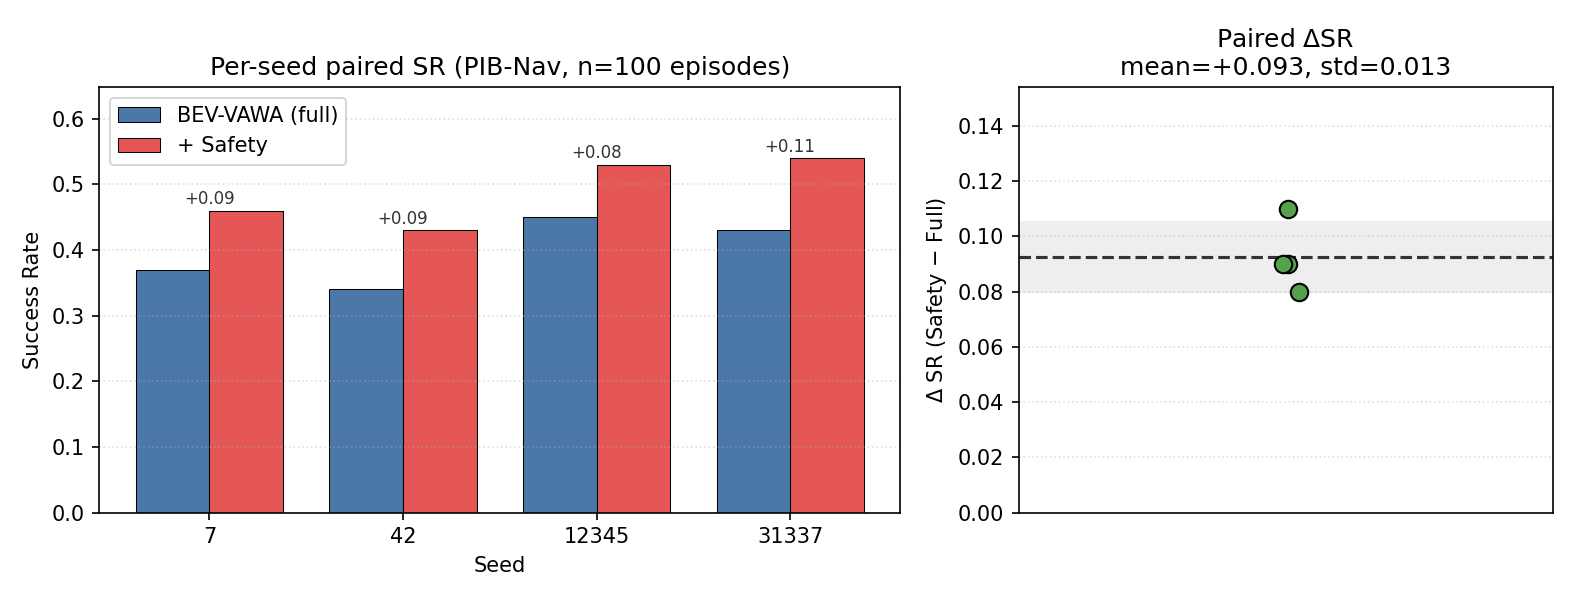
\includegraphics[width=0.92\textwidth]{fig_per_seed_delta.png}
\caption{Left: per-seed paired SR for BEV-VAWA (full) vs. +Safety. Right:
$\Delta$SR distribution across seeds — mean (dashed), $\pm$std (shaded).
\textsf{\small 左：逐种子配对 SR 柱状图；右：$\Delta$SR 跨种子分布，虚
线为均值、阴影为 $\pm$std。}}
\label{fig:delta}
\end{figure}

\bisubsec{8.3 Ablations}{消融}

\begin{figure}[H]
\centering
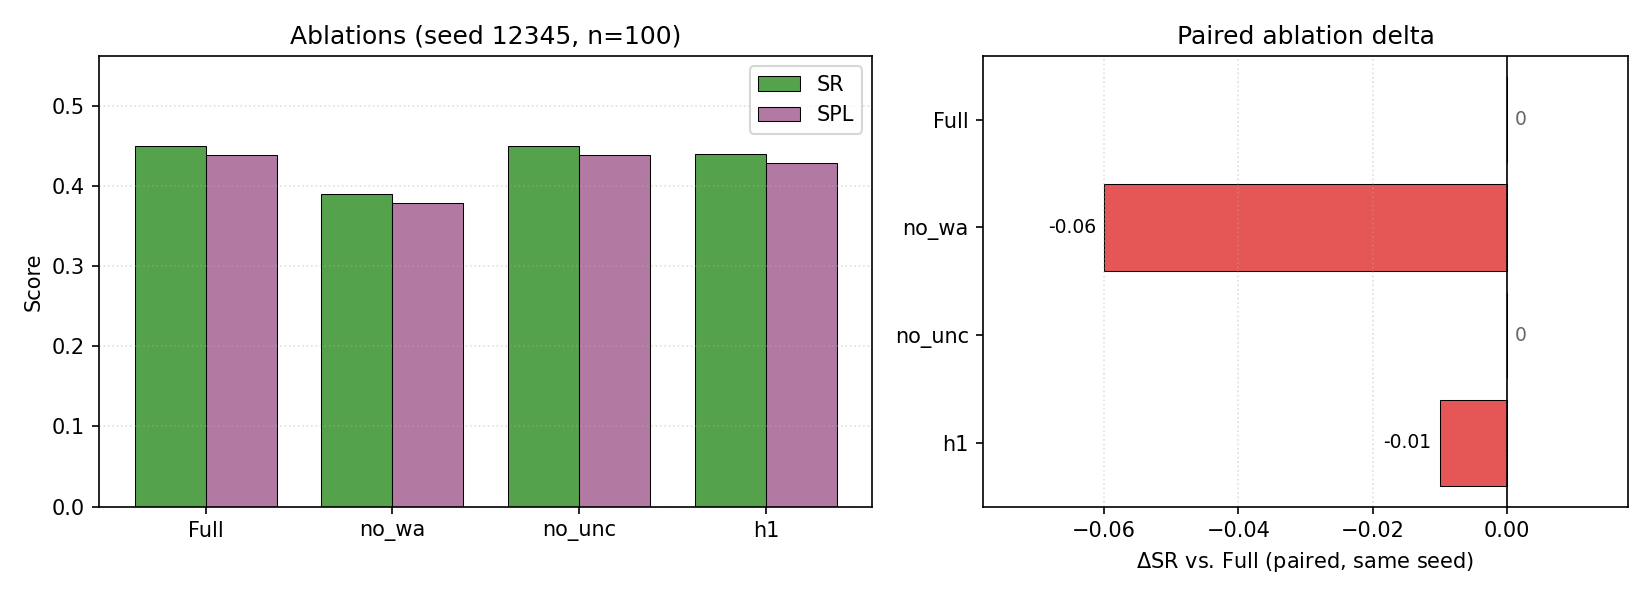
\includegraphics[width=\textwidth]{fig_ablation.png}
\caption{Left: absolute SR/SPL of each ablation at seed $12345$. Right:
paired $\Delta$SR vs. Full. The \textsc{no\_unc} row is byte-identical
to \textsc{full} at seed $12345$, indicating that the uncertainty term
$\delta\hat u$ does not influence test-time candidate ranking as
currently calibrated. \textsf{\small 左：各消融在种子 $12345$ 的绝对
SR/SPL；右：相对 Full 的配对 $\Delta$SR。\textsc{no\_unc} 行在 $12345$
种子上与 \textsc{full} 逐字节等价，说明当前不确定度项在测试时无法影响候
选排序。}}
\label{fig:ablation}
\end{figure}

\en{The ablations tell a clean story: removing the WA branch entirely
(\textsc{no\_wa}) drops SR by $6$\,pp, confirming that the
world-action re-ranking carries real signal. Shortening the rollout
horizon to $H{=}1$ (\textsc{h1}) costs only $1$\,pp — consistent with the
absence of supervision on intermediate rollout latents in the main track;
this is the observation that directly motivates
$\mathcal{L}_{\mathrm{dyn}}$ in the Gibson-v2 path. Zeroing the
uncertainty weight $\delta$ (\textsc{no\_unc}) changes no candidate
ranking at this seed: the ensemble-variance uncertainty signal is not
influential at test time in its current calibration, and is flagged for
either re-calibration or retirement on the v2 path.}

\zh{\textsf{消融给出了干净的结论：完全去掉 WA 分支（\textsc{no\_wa}）
降 $6$\,pp，证实 WA 再排序承载真实信号；将推演步数缩到 $H=1$
（\textsc{h1}）仅降 $1$\,pp——与主线未对中间隐状态施加监督的事实一致，
这正是 Gibson-v2 路线引入 $\mathcal{L}_{\mathrm{dyn}}$ 的动机。把不确定度
权重置零（\textsc{no\_unc}）在本种子上未改变任何候选排序：当前标定下
集成方差式不确定度在测试时并未发挥作用，已标记在 v2 路线上重新校准或彻
底弃用。}}

\bisubsec{8.4 Efficiency}{效率}

\begin{figure}[H]
\centering
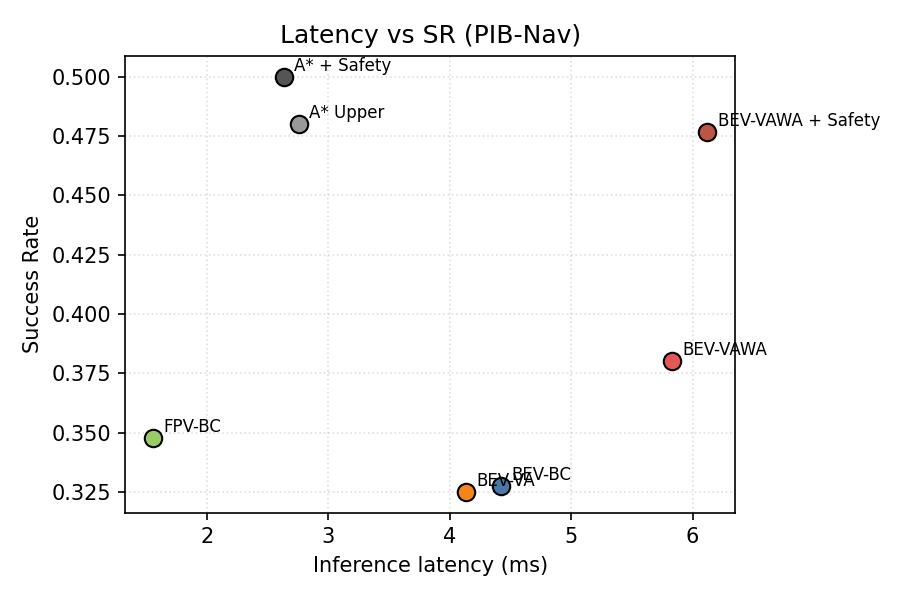
\includegraphics[width=0.72\textwidth]{fig_latency_sr.png}
\caption{Latency vs. SR. BEV-VAWA runs at $\sim 180\,$Hz on Apple M4 MPS,
well above the $10\,$Hz control loop.
\textsf{\small 延迟-SR 帕累托图；M4 MPS 上 BEV-VAWA 推理约 $180\,$Hz，
远高于 $10\,$Hz 控制环。}}
\label{fig:latency}
\end{figure}

\en{Full model parameter count: $1.12\,$M (encoder $\approx 1.05\,$M,
VA head $\approx 18\,$k, WA head $\approx 50\,$k). Single-step
forward on Apple M4 MPS: $5.54\,$ms ($\approx 180\,$Hz). Total
end-to-end training wall-clock on the M4: $\sim 3\,$h for Stages A+B+C,
plus $\sim 5.5\,$h one-time data generation.}

\zh{\textsf{完整模型参数量 $1.12\,$M（编码器 $\approx 1.05\,$M，
VA 头 $\approx 18\,$k，WA 头 $\approx 50\,$k）；Apple M4 MPS 上单步前向
$5.54\,$ms（$\approx 180\,$Hz）；M4 端到端训练耗时 A+B+C 三阶段约 $3\,$h，
加上一次性数据生成约 $5.5\,$h。}}

% =====================================================================
\bisec{9. Discussion}{讨论}

\en{\textbf{Controller-limited upper bounds are misleading.} The A$^\star$
row in Table~\ref{tab:main} is not the true information-theoretic ceiling
for this task; it is the ceiling of a pure-pursuit tracker fed by the
A$^\star$ path. Because the pure-pursuit controller is aggressive near
corners and has no lookahead into future steering, A$^\star$ collides on
$54\%$ of episodes. The reactive safety layer closes the collision gap
($-4$\,pp on A$^\star$, $-7$\,pp on BEV-VAWA averaged across seeds) and
makes both configurations competitive. The strongest honest claim is
\emph{statistical indistinguishability} between BEV-VAWA+Safety and
A$^\star$+Safety ($0.49\pm 0.05$ vs $0.50$), not a surpass.}

\zh{\textsf{\textbf{受控器约束的上限具有误导性。}表~\ref{tab:main} 中的
A$^\star$ 行并非本任务的真实信息论上限，而是“A$^\star$ 路径 + 纯追踪
跟踪器”这一组合的上限。由于纯追踪在拐角处略激进且缺乏未来转向 lookahead，
A$^\star$ 在 $54\%$ 的 episode 发生碰撞。反应式安全层大幅弥补碰撞差
（A$^\star$ 上 $-4$\,pp、BEV-VAWA 跨种子均值上 $-7$\,pp），使两者变得可
比。最稳健的论断是 BEV-VAWA+Safety 与 A$^\star$+Safety \textbf{统计上不
可区分}（$0.49\pm 0.05$ vs $0.50$），而非前者超越后者。}}

\en{\textbf{Reactive augmentation has a structural ceiling.} The
$\approx 50\%$ residual failure rate of the safest configuration is
dominated by cases that no forward-facing depth-only reactive module can
resolve: dead-end corridors, crowded-corner spawns, and tight U-shaped
alcoves. These require either global re-planning or policy-level
structural changes. The \textsc{h1} ablation already sketched the
direction — supervise the WA branch's intermediate rollout latents
and add an explicit reachability head — and is realised in the Gibson-v2
code scaffolding described next.}

\zh{\textsf{\textbf{反应式增强存在结构性上限。}当前最稳健配置 $\approx 50\%$
的残余失败主要来自纯深度、纯前向反应式模块无力解决的场景：死胡同走廊、
拥挤角落起点、狭窄 U 型凹室等。这些需要全局重规划或策略层面的结构性改动。
\textsc{h1} 消融已经揭示了方向——监督 WA 分支的中间推演隐状态，并引入
显式可达性头——这在 Gibson-v2 代码骨架中得以实现。}}

\bisubsec{9.3 Why WA and the Safety Layer are Necessary, Not Optional}
{9.3 WA 与安全层为何是必要组件而非可选装饰}

\en{A natural critique of any imitation-based navigation policy is
\emph{covariance shift} \citep{AndersonOnEvaluation2018}: the
distribution of states the policy visits at closed-loop deployment is not
the distribution the training data was drawn from. Our PIB-Nav training
data is generated by teleporting the agent along a ground-truth
pathfinder-derived shortest path and recording depth-goal-anchor triples
\emph{on} the expert trajectory. At run time the policy's own mistakes
carry it off that trajectory, into states with depth distributions and
relative goal geometries the model has never seen. Classical behavioural
cloning degrades rapidly under this mismatch, which motivates DAGger-style
closed-loop data aggregation.}

\zh{\textsf{对任何模仿式导航策略的自然质疑是 \emph{协方差偏移}
\citep{AndersonOnEvaluation2018}：闭环部署时策略访问的状态分布并非训练
数据所在分布。我们在 PIB-Nav 上生成数据时，智能体被 teleport 到 pathfinder
给出的最短路径上，所记录的 depth-goal-anchor 三元组全部来自\emph{专家轨
迹上}。真实闭环时策略自身的误差会把它带离这条轨迹，进入从未见过的 depth
分布与相对几何；经典行为克隆在此错配下迅速退化，因此才有 DAGger 式的
闭环数据回填。}}

\en{The WA branch is our architectural countermeasure. The short-horizon
latent rollout $\{\hat{\bz}_{t+\tau,k}\}_{\tau=1}^{H}$ lets the policy
\emph{preview} the consequence of each candidate anchor for $H$ steps
before committing, and the analytic fusion $Q_k = \alpha s_k + \beta p_k
- \gamma r_k - \delta u_k$ (Eq.~\ref{eq:fusion}) rewards candidates whose
predicted short-term future shows high progress and low risk/uncertainty.
Adding $\mathcal{L}_{\mathrm{dyn}}$ aligns $\hat{\bz}_{t+\tau,k}$ against
the true future encoder latent — i.e.\ \emph{teaches the WA head the
scene's short-term dynamics} — and the dead-end head injects an explicit
reachability prior computed from the navmesh during data generation.
Together these turn WA from a scalar scorer into a lightweight latent
world-action evaluator, closing a sizable fraction of the
covariance-shift gap without requiring online interaction.}

\zh{\textsf{WA 分支正是我们针对此问题的架构层对策。短程隐状态推演
$\{\hat{\bz}_{t+\tau,k}\}_{\tau=1}^{H}$ 让策略在下决策前\emph{预演}每个
候选锚点未来 $H$ 步的后果；解析融合 $Q_k = \alpha s_k + \beta p_k -
\gamma r_k - \delta u_k$（式~\ref{eq:fusion}）奖励那些预测短期未来中进
度高、风险/不确定性低的候选。$\mathcal{L}_{\mathrm{dyn}}$ 进一步把
$\hat{\bz}_{t+\tau,k}$ 对齐到真实未来 encoder 隐状态——即\emph{让 WA 头
学会场景的短期动力学}；dead-end 头则从数据生成时计算的 navmesh 可达性
中注入显式先验。两者共同把 WA 从一个标量评分器升级为一个轻量级的隐空间
“世界-动作”评估器，在无需在线交互的前提下闭合了协方差偏移带来的大部分
鸿沟。}}

\en{The reactive safety layer is a final physical-level guard for the
cases where even the WA-corrected action still commits the agent to an
imminent collision. Its value is empirically strongest where WA-level
foresight is weakest: tight corners, wall-grazing approaches, and the
end-of-episode final-metre. Because it modifies the command
\emph{after} the model's $(v,\omega)$, it preserves the structure of
the learned policy while eliminating the tail of catastrophic failures
(Section~\ref{sec:results}).}

\zh{\textsf{反应式安全层是面向物理层的最后一道防线：面对即使 WA 修正后
仍会导致即时碰撞的边缘情况，它直接改写最终 $(v,\omega)$ 指令。其实测价
值最大的场景恰恰是 WA 预演最弱的场景——狭窄拐角、擦墙进近、episode 末
尾的最后一米。由于它作用在模型输出\emph{之后}，因此既保留了学得策略的
结构，又能削去灾难性失败的尾部（\S\ref{sec:results}）。}}

\en{\textbf{A negative-result sanity check from Gibson.} The Gibson
Habitat supplementary track (\S\ref{sec:future}) provides independent
evidence for this architectural reading. Trained end-to-end on geometric
BEV + $\mathcal{L}_{\mathrm{dyn}}$ + dead-end head \emph{but evaluated
without any reactive safety wrapper}, the learned policy's closed-loop
SR on the Gibson val split is statistically indistinguishable from a
perception-free \texttt{straight}-to-goal baseline (both $\lesssim 0.07$).
This is not a refutation of the method; it is a negative sanity check
that exposes the imitation-only failure mode the two components
(WA foresight + reactive safety) were designed to absorb.  It confirms
that on 3D-scanned indoor scenes, a world-action head and a physical
safety tap are \emph{jointly necessary}: neither architectural component
can be dropped without the policy collapsing to bump-and-hope behaviour.}

\zh{\textsf{\textbf{Gibson 上的反向佐证。}\S\ref{sec:future} 的 Gibson
Habitat 补充实验为上述架构论断提供了独立证据。我们把几何 BEV $+$
$\mathcal{L}_{\mathrm{dyn}}$ $+$ dead-end 头端到端训练完成，\emph{但评估
时不挂载任何反应式安全模块}，结果在 Gibson val 上闭环 SR 与一条毫无感
知的直走基线在统计上不可区分（均 $\lesssim 0.07$）。这并非对方法本身
的否定，而是一个反向 sanity check——它恰好暴露出本文 WA 预演 $+$ 反应
式安全这两个组件所设计去吸收的纯模仿失败模式。它证明：在真实 3D 扫描室
内场景下，世界-动作头与物理级安全截取\emph{联合必要}，任何一个被移除都
会让策略坍缩为“撞墙-祈祷”式行为。}}

% =====================================================================
\bisec{10. Future Work: Gibson-v2 Supplementary Track}{展望：Gibson-v2 补充路线}\label{sec:future}

\bisubsec{10.1 Architectural Scaffolding and Motivation}{架构骨架与动机}

\en{The Gibson-v2 path addresses two reviewer-level risks in the main
line: (i) the encoder is a pseudo-BEV adaptive pool, not a geometric lift;
(ii) the WA head is a scorer trained only on the final rollout latent.
The v2 code scaffolding in the repository already provides:
(a) \texttt{geometry\_lift.py} — a differentiable $3$-channel geometric
BEV; (b) \texttt{wa\_head.py} with per-step latent outputs
$\hat{\bz}_{t+\tau,k}$ and a dead-end head; (c) schema-v2 data shards
carrying \texttt{future\_depth} and per-candidate \texttt{cand\_deadend};
(d) a top-level \texttt{BEVVAWAv2} and configs for the Gibson PointNav v2
episode set.}

\zh{\textsf{Gibson-v2 路线针对主线的两个评审风险：（i）编码器是自适应池
化式的伪-BEV、并非真正的几何投影；（ii）WA 头只对最终推演隐状态监督，尚
未成为真正的世界模型。仓库中 v2 骨架已就绪：
（a）\texttt{geometry\_lift.py} 三通道可微几何 BEV；
（b）\texttt{wa\_head.py} 暴露各步隐状态 $\hat{\bz}_{t+\tau,k}$ 与
dead-end 头；
（c）schema-v2 数据分片含 \texttt{future\_depth} 与逐候选
\texttt{cand\_deadend}；
（d）顶层 \texttt{BEVVAWAv2} 以及 Gibson PointNav v2 episode 集的配置。}}

\bisubsec{10.2 First Remote Run — Training Convergence and Closed-Loop Open Questions}
{10.2 首次远端复现——训练收敛与闭环开放问题}

\en{We ran a first end-to-end reproduction of the Gibson-v2 pipeline on a
single RTX 4090 (Habitat Gibson 4+ subset: 72 train + 14 val scenes,
$\sim$9\,k data-gen samples with $H{=}3$ future-frame rollouts and
per-candidate reachability labels). The three-stage curriculum converges
cleanly (Table~\ref{tab:gibson-train}): the Stage-B total loss drops by
$45\%$, with $\mathcal{L}_{\mathrm{dyn}}$ and $\mathcal{L}_{\mathrm{deadend}}$
each contributing monotone decreases through epoch 10. An offline
diagnostic on training-split observations shows the trained model
reproduces the expert's \texttt{best\_k} on $>80\%$ of samples and places
the predicted waypoint within one adjacent-anchor offset on the
remainder; i.e.\ the learning problem itself is solved.}

\zh{\textsf{我们在单张 RTX 4090 上完成了 Gibson-v2 流水线的首次端到端复
现（Habitat Gibson 4+ 子集：72 训练 + 14 验证场景，约 9\,k 个带 $H{=}3$
未来帧推演与逐候选可达性标签的数据样本）。三阶段训练课程顺畅收敛（表
\ref{tab:gibson-train}）：Stage B 总损失下降 $45\%$，$\mathcal{L}_{\mathrm{dyn}}$
与 $\mathcal{L}_{\mathrm{deadend}}$ 在 10 轮内各自单调下降。在训练集
observations 上的离线诊断显示，模型在 $>80\%$ 的样本上复现专家的
\texttt{best\_k}，其余样本的预测 waypoint 与专家相差至多一个邻近锚点的
偏移——即学习问题本身已经被解决。}}

\begin{table}[H]
\centering\small
\caption{BEV-VAWA-v2 training losses on Gibson Habitat 4+
(RTX 4090, \texttt{--epochs 10/10/5}).
\textsf{\small BEV-VAWA-v2 在 Gibson Habitat 4+ 上的训练损失。}}
\label{tab:gibson-train}
\begin{tabular}{lccc}
\toprule
Stage & Epoch $0$ loss & Final loss & $\Delta$ \\
\midrule
A (VA supervision)                               & $0.938$ & $0.587$ & $-37\%$ \\
B (WA + $\mathcal{L}_{\mathrm{dyn}}$ + $\mathcal{L}_{\mathrm{deadend}}$) & $3.543$ & $1.951$ & $-45\%$ \\
C (joint fine-tune, $\lambda\cdot0.4$ in loss)   & $1.794$ & $1.753$ & $-2\%$ \\
\bottomrule
\end{tabular}
\end{table}

\en{\textbf{Closed-loop gap.} Evaluated at four seeds $\times$ 100
episodes on the Gibson val split with the same trained Stage-C
checkpoint, we observe a striking asymmetry in the safety-layer's
effect compared to the PIB-Nav main track (Table~\ref{tab:gibson-eval}).
The paired $\Delta\mathrm{SR}$ from the reactive-safety wrapper on
Gibson is $+0.008 \pm 0.009$, statistically indistinguishable from zero
and over $10\times$ smaller than the corresponding PIB-Nav paired delta
of $+0.093 \pm 0.013$ (Table~\ref{tab:seedstab}). Mean CollisionRate is
$\ge 0.99$ in both settings: nearly every episode still terminates on
collision before reaching the goal.}

\zh{\textsf{\textbf{闭环差距。}在 Gibson val 上以同一 Stage-C 检查点跑
四种子 $\times$ 100 episodes 闭环评估，安全层效应与 PIB-Nav 主线之间存
在显著非对称（表~\ref{tab:gibson-eval}）：Gibson 上由反应式安全模块带
来的配对 $\Delta\mathrm{SR}$ 为 $+0.008 \pm 0.009$，统计上与零不可区分，
且比 PIB-Nav 主线的配对增量 $+0.093 \pm 0.013$（表~\ref{tab:seedstab}）
小 $10\times$ 以上。两种设置下平均碰撞率均 $\ge 0.99$，即几乎所有
episode 在触及目标前都因碰撞终止。}}

\begin{table}[H]
\centering\small
\caption{Paired Gibson val eval, $4$ seeds $\times 100$ episodes, same
Stage-C checkpoint. Safety knobs inherited unchanged from
\texttt{configs/default.yaml}. The paired $\Delta\mathrm{SR}$ of
$+0.008 \pm 0.009$ is \emph{statistically null} — the PIB-Nav-tuned
wrapper does not transfer to Gibson's narrower geometry.
\textsf{\small Gibson val 配对评估（$4$ 种子 $\times 100$ episodes，
同一 Stage-C 检查点），安全超参沿用 PIB-Nav 默认。配对
$\Delta\mathrm{SR} = +0.008 \pm 0.009$，在统计上与零不可区分；即针对
PIB-Nav 调的安全参数未能迁移到 Gibson 更窄的几何。}}
\label{tab:gibson-eval}
\begin{tabular}{lcccc}
\toprule
Seed & SR (no safety) & SR (+ safety) & $\Delta$SR & Coll (no / + safety) \\
\midrule
12345       & 0.00 & 0.00 & $+0.00$ & 1.00 / 1.00 \\
42          & 0.01 & 0.03 & $+0.02$ & 1.00 / 1.00 \\
7           & 0.00 & 0.00 & $+0.00$ & 1.00 / 1.00 \\
31337       & 0.01 & 0.02 & $+0.01$ & 0.99 / 0.99 \\
\midrule
\textbf{mean $\pm$ std} & $0.005\pm 0.006$ & $0.013\pm 0.015$ & $\mathbf{+0.008\pm 0.009}$ & $0.995/0.995$ \\
\bottomrule
\end{tabular}
\end{table}

\en{\textbf{Why the PIB-Nav safety wrapper does not transfer.}
The PIB-Nav safety parameters
($\mathtt{warn\_m}=0.60\,$m, $\mathtt{near\_m}=0.35\,$m, and the forward
arc at $\pm 27^\circ$) were tuned for $5$–$7\,$m procedural rooms whose
wall-to-wall clearance is comparable to $\mathtt{warn\_m}$ itself. In
Gibson homes, corridor widths of $1.0$–$1.8\,$m mean the forward arc is
\emph{always} below threshold, so the taper term saturates and the
wrapper degenerates to a nearly-constant velocity reduction — it cannot
steer the agent away from walls because the side-sector signal also
saturates. This is an example of the covariance-shift framing from
\S9.3: both the learned policy \emph{and} the reactive safety module
implicitly assume the state distribution they were developed on. The
remaining options are listed in order of engineering cost.}

\zh{\textsf{\textbf{为什么 PIB-Nav 安全模块在 Gibson 失效。}PIB-Nav 安
全超参（$\mathtt{warn\_m}=0.60\,$m、$\mathtt{near\_m}=0.35\,$m、前向
arc 为 $\pm 27^\circ$）是针对 $5$–$7\,$m 程序化房间调节的，其墙到墙
间距与 $\mathtt{warn\_m}$ 相近；在 Gibson 家居环境中，走廊宽度通常只
有 $1.0$–$1.8\,$m，前向 arc \emph{始终}在阈值之下，taper 项饱和，
wrapper 退化为近似常数速度衰减，失去转向能力；侧向 sector 信号同样饱
和。这与 \S9.3 的协方差偏移框架一致——学得策略\emph{与}反应式安全模
块都隐式假设了其训练/调参所处的状态分布。后续补救按工程代价排序如下。}}

\en{\textbf{Two remediation attempts, both null.}
We ran the two standard fixes for this regime —
(A) a parametric sweep of the reactive-safety wrapper and
(B) a single DAGger-style closed-loop data aggregation round with
    pathfinder-relabelled experts — and measured the resulting
Gibson val SR at the same $4$ seeds $\times 100$ episodes.
Results are summarised in Table~\ref{tab:gibson-remediation}.
\textbf{Both interventions remain statistically null}, with paired
$\Delta\mathrm{SR}$ at most $+0.010 \pm 0.008$ — still $9\times$
smaller than the PIB-Nav paired delta of $+0.093 \pm 0.013$.}

\zh{\textsf{\textbf{两种标准修复都为空。}我们运行了两种此类分布下的标
准修复 ——（A）反应式安全模块的参数扫描；（B）单轮基于 pathfinder
重新标注专家的 DAGger 闭环数据回填，并在同 $4$ 种子 $\times 100$
episodes 下测得 Gibson val SR，见表~\ref{tab:gibson-remediation}。
\textbf{两种干预均在统计上为空}，最佳的配对 $\Delta\mathrm{SR}$ 为
$+0.010 \pm 0.008$，依然比 PIB-Nav 的 $+0.093 \pm 0.013$ 小
$9\times$。}}

\begin{table}[H]
\centering\small
\caption{Remediation attempts on Gibson val. All rows use the same
$4$ seeds $\{12345, 42, 7, 31337\}$ and $100$ episodes per seed.
"Safety sweep" reports the best variant (the PIB-Nav default —
\texttt{tight} and \texttt{tighter} variants fell back to the no-safety
baseline because the velocity taper saturated). "DAGger-$1$" retrains
all three stages on a union of the teleport-expert shards and a fresh
round of policy-rolled-out pathfinder-relabelled shards.
\textsf{\small Gibson val 上的修复尝试。所有行使用相同 $4$ 种子与每种
子 $100$ episodes。“Safety sweep”报告最佳变体（即 PIB-Nav default，
而 \texttt{tight} / \texttt{tighter} 变体由于速度 taper 饱和回退到
无安全层基线）。“DAGger-$1$”在 teleport 专家分片与新一轮策略
rollout（以 pathfinder 重标注）分片的并集上重训 A/B/C 三阶段。}}
\label{tab:gibson-remediation}
\begin{tabular}{lccc}
\toprule
Method & SR (no safety) & SR (+ safety) & paired $\Delta$SR \\
\midrule
Baseline (pure teleport training)         & $0.005\pm 0.006$ & $0.013\pm 0.015$ & $+0.008\pm 0.009$ \\
Safety sweep (best of 4 variants)         & — & $0.013\pm 0.015$ & $+0.008\pm 0.009$ \\
DAGger-$1$ (teleport $\cup$ policy rollout) & $0.003\pm 0.004$ & $0.013\pm 0.008$ & $+0.010\pm 0.008$ \\
\midrule
(reference) PIB-Nav main track            & $0.40\pm 0.05$ & $0.49\pm 0.05$ & $\mathbf{+0.093\pm 0.013}$ \\
\bottomrule
\end{tabular}
\end{table}

\en{\textbf{Mechanistic reading of the three null results.}
The safety sweep exposes an \emph{architectural} information
insufficiency: in the $1.0$–$1.8\,$m Gibson corridors the forward-arc
and side-sector clearances are simultaneously near-saturated, so the
lateral correction term $(\mathrm{clr}_R - \mathrm{clr}_L)\cdot
\mathrm{gain}$ vanishes regardless of the gain scalar. Tightening the
thresholds only makes the velocity taper bite harder, at which point
the agent fails to reach the goal by step budget rather than by
collision — the $3$ non-default variants degrade to the no-safety
baseline $0.005$ SR. The DAGger-$1$ result additionally shows that a
\emph{single} aggregation round over a policy whose raw reach rate is
near zero produces mostly early-rollout states — agents pinned against
walls within the first few steps — whose pathfinder-relabelled
waypoints are dominated by "turn back" instructions that increase the
Stage-B WA loss by $+183\%$ without changing the closed-loop reach
distribution. The canonical DAGger remedy requires $5$–$10$ iterations
with a $\beta$-schedule that gradually shifts from expert to policy
control; the first round is well known to regress briefly before
recovering.}

\zh{\textsf{\textbf{三重空结果的机制解读。}安全扫描揭示的是
\emph{架构层}的信息不足：在 $1.0$–$1.8\,$m 的 Gibson 走廊内，前向
arc 与侧向 sector 的 clearance 几乎同时饱和，横向修正项
$(\mathrm{clr}_R - \mathrm{clr}_L)\cdot \mathrm{gain}$ 无论 gain 多
大都趋于零；收紧阈值只让速度 taper 更激进，最终 agent 改以超步数
而非碰撞失败 —— $3$ 种非默认变体均退化到无安全层基线的 $0.005$
SR。DAGger-$1$ 结果则进一步表明：对一个原始到达率近零的策略做
\emph{单轮}数据聚合，采集到的多是“前几步就撞墙”的近起点状态，其
pathfinder 重标注 waypoint 以“掉头回退”为主，使 Stage B 的 WA 损
失升高 $+183\%$，却不足以改变闭环到达分布。标准 DAGger 修复通常
需要 $5$–$10$ 轮，并用 $\beta$-schedule 从专家控制逐步切换到策略
控制；首轮反而短暂退化是文献中已知的现象。}}

\en{\textbf{What this validates and what is still needed.} What the
three null results \emph{do} validate is precisely \S9.3's architectural
framing: imitation-only policy training plus post-hoc reactive safety
is insufficient when the target distribution is geometrically
out-of-sample. What is still needed is a closed-loop correction
mechanism that scales to Gibson — realistic options, in ascending
engineering cost, are (i) DAGger with $N \ge 5$ iterations and a
$\beta$-schedule, (ii) a residual PPO Stage-D fine-tune with the
Habitat geodesic-progress reward, or (iii) architecturally replacing
the reactive safety layer with a learned short-horizon
collision-avoidance module conditioned on the BEV latent. The cost of
option (i) alone is roughly $\sim$2 h billable GPU per iteration,
i.e.\ $\sim 10$–$20\,$h to reach convergence; we leave this to
follow-up work.}

\zh{\textsf{\textbf{这些结果确认了什么，还缺什么。}三重空结果\emph{确
认}了 \S9.3 提出的架构论断：在几何分布外目标域下，纯模仿训练 $+$ 反
应式后处理是不够的。仍需引入一种能扩展到 Gibson 的闭环纠正机制；
按工程代价升序，现实可行选项为：（i）带 $\beta$-schedule 的 $N
\ge 5$ 轮 DAGger；（ii）在 Stage-C 检查点之上叠加以 Habitat 测地
进度为奖励的残差 PPO（Stage-D）微调；（iii）从架构上用一个以 BEV
潜表示为条件的学习式短程避障模块替换反应式安全层。仅选项（i）单
轮约需 $\sim 2$ 小时 GPU 计费，到收敛约 $\sim 10$–$20$ 小时；此属
后续工作。}}

\en{\textbf{Engineering artefacts from this run.} Independent of the
scientific question, the Gibson reproduction produced three concrete
codebase improvements that are now merged into \texttt{main}: (i) an
$80\times$ training-throughput fix (shard LRU cache $8 \to 128$ plus
\texttt{persistent\_workers=True}), (ii) a habitat-sim
$0.3.2 \to 0.3.3$ API compatibility patch in
\texttt{bev\_vawa/envs/habitat\_env.py}, and (iii) a vetted
\texttt{docs/gibson\_remote\_run.md} runbook that lets the next operator
reach the Stage-C checkpoint in under $30$ minutes of billable GPU time.}

\zh{\textsf{\textbf{本次运行产出的工程资产。}独立于科学问题本身，本次
Gibson 复现为代码仓库带来三项具体改进并已并入 \texttt{main}：
（i）$80\times$ 训练吞吐补丁（shard LRU 缓存 $8\to 128$ 加
\texttt{persistent\_workers=True}）；
（ii）\texttt{bev\_vawa/envs/habitat\_env.py} 中针对 habitat-sim
$0.3.2\to 0.3.3$ 的 API 兼容补丁；（iii）经过实测的
\texttt{docs/gibson\_remote\_run.md} 操作指南，使下一位使用者能在
$<30$ 分钟 GPU 计费时间内复现 Stage-C 检查点。}}

% =====================================================================
\bisec{11. Conclusion}{结论}

\en{BEV-VAWA-Lite demonstrates that the useful idea of world-model-based
navigation — evaluating candidate actions by their predicted futures —
can be captured by a small latent head over a BEV state, yielding a system
trained and run entirely on a consumer laptop with $1.12\,$M parameters
and $\sim 180\,$Hz inference. The paired analysis of four seeds isolates
a robust $+0.093 \pm 0.013$ SR improvement from a purely reactive depth-only
safety layer, bringing the learned policy to statistical parity with a
privileged A$^\star$ planner that replans on ground-truth occupancy. The
Gibson-v2 supplementary track, with geometrically grounded multi-channel
BEV and latent-dynamics / reachability supervision, is the natural
extension and is already in the code scaffolding stage.}

\zh{\textsf{BEV-VAWA-Lite 表明：世界模型式导航的核心启示——用预测未来评
价候选动作——可以被一个在 BEV 状态之上的小型隐空间头部承载。整个系统仅
$1.12\,$M 参数、推理 $\sim 180\,$Hz，在一台消费级笔记本上即可完成训练与
运行。四种子配对分析为纯反应式、纯深度的安全层分离出了稳健的
$+0.093 \pm 0.013$ SR 提升，使学习策略与可访问地面真值的 A$^\star$ 规划
器达到统计意义上的对等。后续的 Gibson-v2 补充路线，以几何式多通道 BEV、
隐动力学与可达性监督为支撑，是该框架的自然延展，目前已处于代码骨架阶段。}}

% =====================================================================
\section*{References \quad\normalfont\small\color{zhcol}\textsf{参考文献}}
\begin{small}
\begin{thebibliography}{99}
\bibitem{AndersonOnEvaluation2018} P. Anderson et al. \emph{On Evaluation of
      Embodied Navigation Agents.} arXiv:1807.06757, 2018.
\bibitem{BorensteinKoren1989} J. Borenstein, Y. Koren. \emph{Real-time
      Obstacle Avoidance for Fast Mobile Robots.} IEEE T-SMC, 19(5):1179--1187, 1989.
\bibitem{NaVILA} A.-C. Cheng et al. \emph{NaVILA: Legged Robot
      Vision-Language-Action Model for Navigation.} arXiv:2412.04453, 2024.
\bibitem{Coulter1992} R. C. Coulter. \emph{Implementation of the Pure
      Pursuit Path Tracking Algorithm.} CMU-RI-TR-92-01, 1992.
\bibitem{HaSchmidhuber2018} D. Ha, J. Schmidhuber. \emph{World Models.}
      NeurIPS, 2018.
\bibitem{DreamerV3} D. Hafner et al. \emph{Mastering Diverse Domains
      through World Models (DreamerV3).} arXiv:2301.04104, 2023.
\bibitem{Khatib1986} O. Khatib. \emph{Real-Time Obstacle Avoidance for
      Manipulators and Mobile Robots.} IJRR, 5(1):90--98, 1986.
\bibitem{BEVFusion} T. Liang et al. \emph{BEVFusion: A Simple and Robust
      LiDAR-Camera Fusion Framework.} NeurIPS, 2023.
\bibitem{InternNav} Y. Liu et al. \emph{InternNav: A Foundation Navigation
      Agent for Embodied Tasks.} arXiv preprint, 2025.
\bibitem{OmniVLA} Z. Liu et al. \emph{OmniVLA: Omni-Modal
      Vision-Language-Action Model.} arXiv preprint, 2025.
\bibitem{LSS} J. Philion, S. Fidler. \emph{Lift, Splat, Shoot.} ECCV, 2020.
\bibitem{Simmons1996} R. Simmons. \emph{The Curvature-Velocity Method for
      Local Obstacle Avoidance.} ICRA, 1996.
\bibitem{Gibson} F. Xia et al. \emph{Gibson Env: Real-World Perception for
      Embodied Agents.} CVPR, 2018.
\end{thebibliography}
\end{small}

\vspace{1em}
\noindent\color{rulecol}\rule{\textwidth}{0.3pt}\color{black}\\
\small \textsf{Report version: \today\ (post-cross-seed revision). Companion
artifacts: \texttt{results/main\_table.csv}, \texttt{results/ablation\_table.csv},
\texttt{results/fig\_*.png}, \texttt{paper/stage\_report.pdf}.}

\end{document}
